\begin{frame}
  \frametitle{ Table of Contents}
  \begin{itemize}
    \item Introduction
    \item Automation and Labor
      \begin{itemize}
        \item Net Impact on Job Market
        \item Solutions to Impeding Problems
      \end{itemize}
    \item Ethical Questions in Automation
      \begin{itemize}
        \item Responsibility in Automated Systems
        \item Trust in Automated Systems
      \end{itemize}
    \item Questions
  \end{itemize}
\end{frame}


\begin{frame}
  \frametitle{ Ethical Automation: Introduction}
  \begin{itemize}
    \item A note on Labor
    \item A brief review of the industrial revolution(s)
    \item The Big Questions:
      \begin{itemize}
        \item We know automation destroys jobs.  How many does it make?
        \item What do we do when people lose their jobs?
      \end{itemize}
  \end{itemize}
\end{frame}


\begin{frame}
  \frametitle{ Ethical Automation: will automation create net job loss?}
  \begin{itemize} 
    \item
  \end{itemize}
\end{frame}


\begin{frame}
  \frametitle{ Ethical Automation: proposed solutions to job loss}
  \begin{itemize}
    \item
  \end{itemize}
\end{frame}

\begin{frame}
  \frametitle{ Ethical Automation: A brief aside}
  \begin{itemize}
    \item From Worker to Product
      \begin{itemize}
        \item We've talked about a worker being replaced by a machine
        \item How do we talk about those machines?
      \end{itemize}
    \item What is Responsibility?
    \item The Big Questions:
      \begin{itemize}
        \item When an automated machine fails, who is responsible?
        \item What kind of failure is acceptable?
      \end{itemize}
  \end{itemize}
\end{frame}


\begin{frame}
  \frametitle{ Ethical Automation: Responsibility in Automation}
  \Large{Responsiblity}
\end{frame}


\begin{frame}
  \frametitle{ Ethical Automation: Responsibility in Automation}
  {\Large Self-Driving Cars}
  \begin{itemize}
    \item The manufacturer is liable for failure, not the user
  \end{itemize}
\end{frame}


\begin{frame}
  \frametitle{ Ethical Automation: Responsibility in Automation}
  {\Large How Safe is Safe Enough?}\\
  424,331 autonomous miles. . . with a catch
  \begin{itemize}
    \item ``Safety Driver''
    \item Relinquished Control
    \item Emergency Intervention
  \end{itemize}
\end{frame}


\begin{frame}
  \frametitle{ Ethical Automation: Trust in Automation}
  \Large{Is it Moral to Trust the Morality of a Machine?}
\end{frame}


\begin{frame}
  \frametitle{ Ethical Automation: Trust in Automation}
  \begin{figure}[bht]
    \centering
    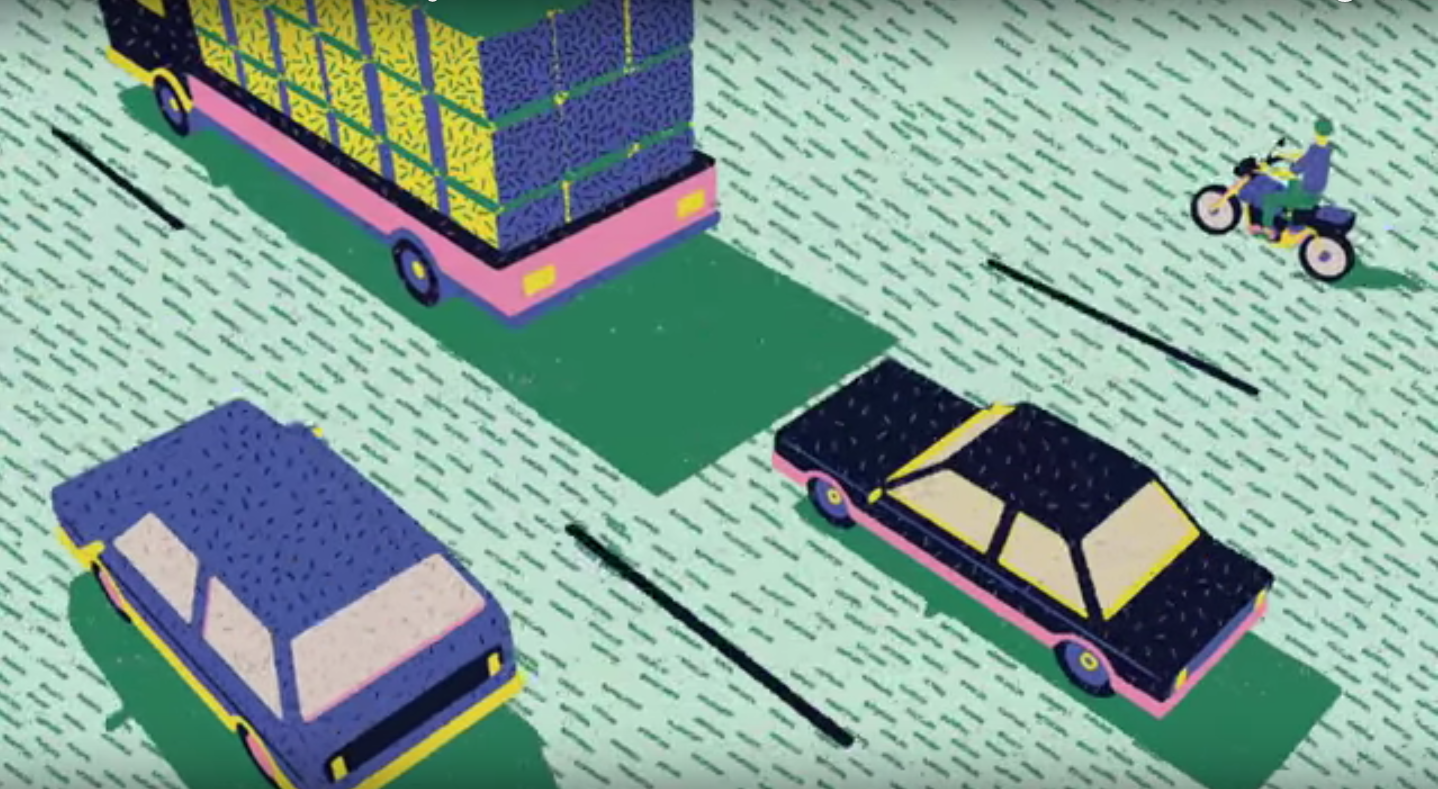
\includegraphics[width=4.0in]{diagrams/image00}
    \caption{An Ethical Scenario.}
  \end{figure}
\end{frame}


\begin{frame}
  \frametitle{ Ethical Automation: Trust in Automation}
  {\Large Reaction vs Decision}
  \begin{itemize}
    \item Humans react while machines decide
  \end{itemize}
\end{frame}


\begin{frame}
  \frametitle{ Ethical Automation: Trust in Automation}
  \begin{figure}[bht]
    \centering
    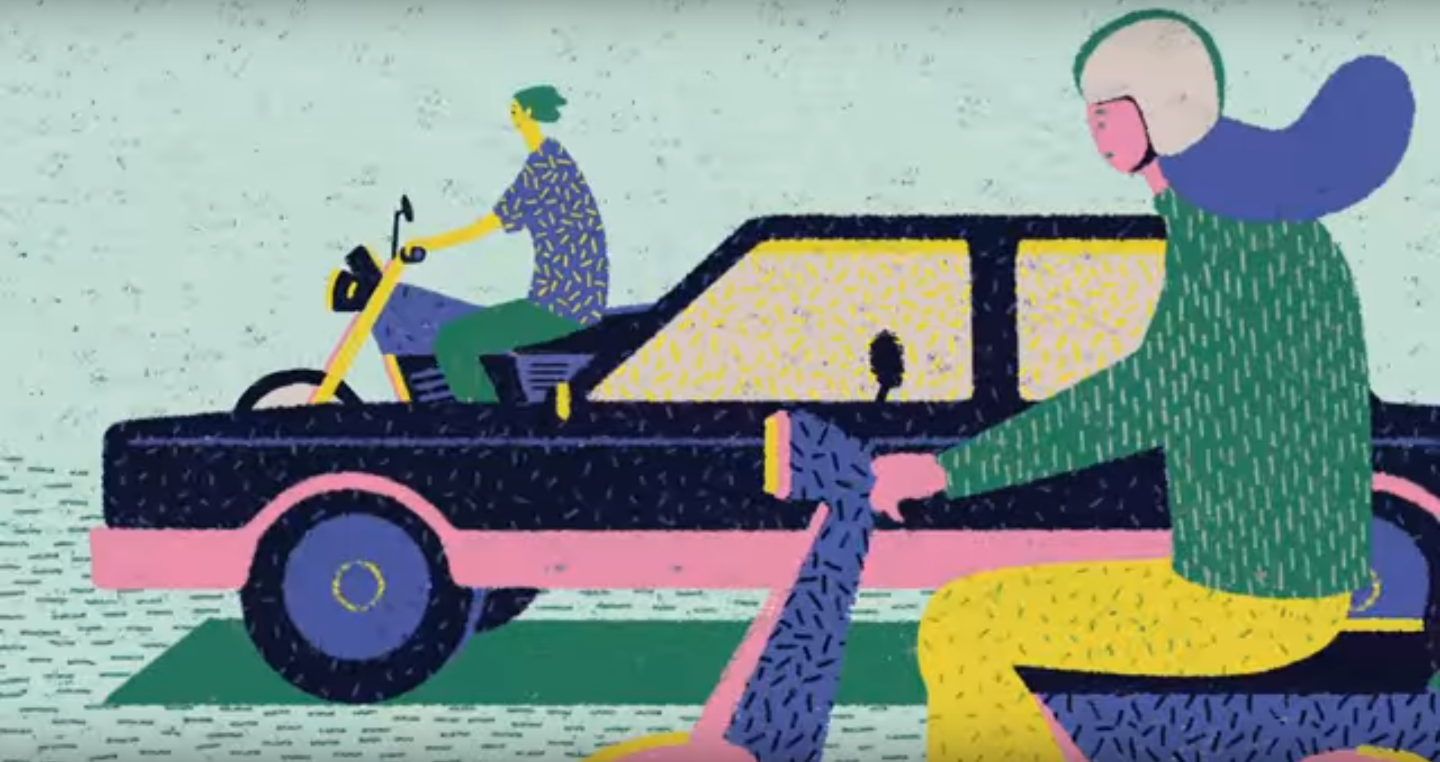
\includegraphics[width=4in]{diagrams/image01}
  \end{figure}
\end{frame}


\begin{frame}
  \frametitle{ Ethical Automation: Trust in Automation}
  {\Large Conclusion}
  \begin{itemize}
    \item These moral dilemmas are too complicated and too controversial to decide
  \end{itemize}
\end{frame}


\begin{frame}
  \frametitle{ Ethical Automation}
\end{frame}


\begin{frame}
  \frametitle{ Ethical Automation: Responsibility in Automation}
  {\Large Self-Driving Cars}
  \begin{itemize}
    \item Do you watch cop shows, crime drama and action flicks?
  \end{itemize}
\end{frame}

\begin{frame}
  \frametitle{ Ethical Automation: Responsibility in Automation}
  {\Large Reaction time!}
  \begin{itemize}
    \item Human reaction time is 2.3 seconds
    \item Airplane 45 seconds
    \item Car 2.3 seconds
  \end{itemize}
\end{frame}

\begin{frame}
  \frametitle{ Ethical Automation: Responsibility in Automation}
  {\Large This is not enough time for;}
  \begin{itemize}
    \item A human to realize something is wrong.
    \item Decide what to do
    \item Take over control
    \item Take action
  \end{itemize}
\end{frame}

\begin{frame}
  \frametitle{ Ethical Automation: Trust in Automation}
  {\Large Driver or AI?}
  \begin{figure}[bht]
    \centering
    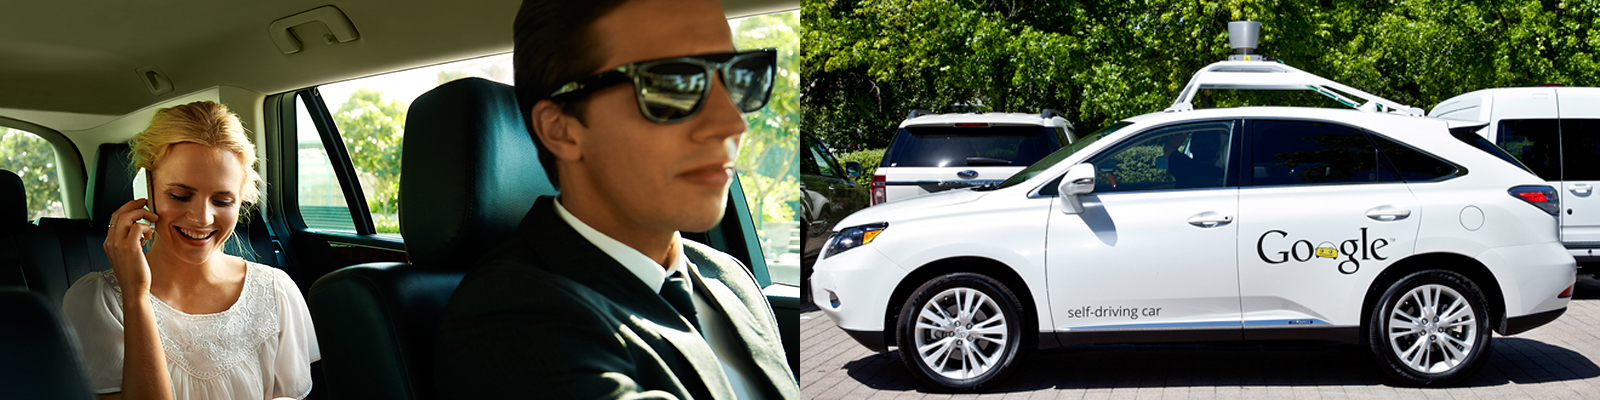
\includegraphics[width=4.0in]{diagrams/car}
  \end{figure}
\end{frame}

\begin{frame}
  \frametitle{ Ethical Automation: Trust in Automation}
  {\Large Mass paranoia?}
  \begin{figure}[bht]
    \centering
    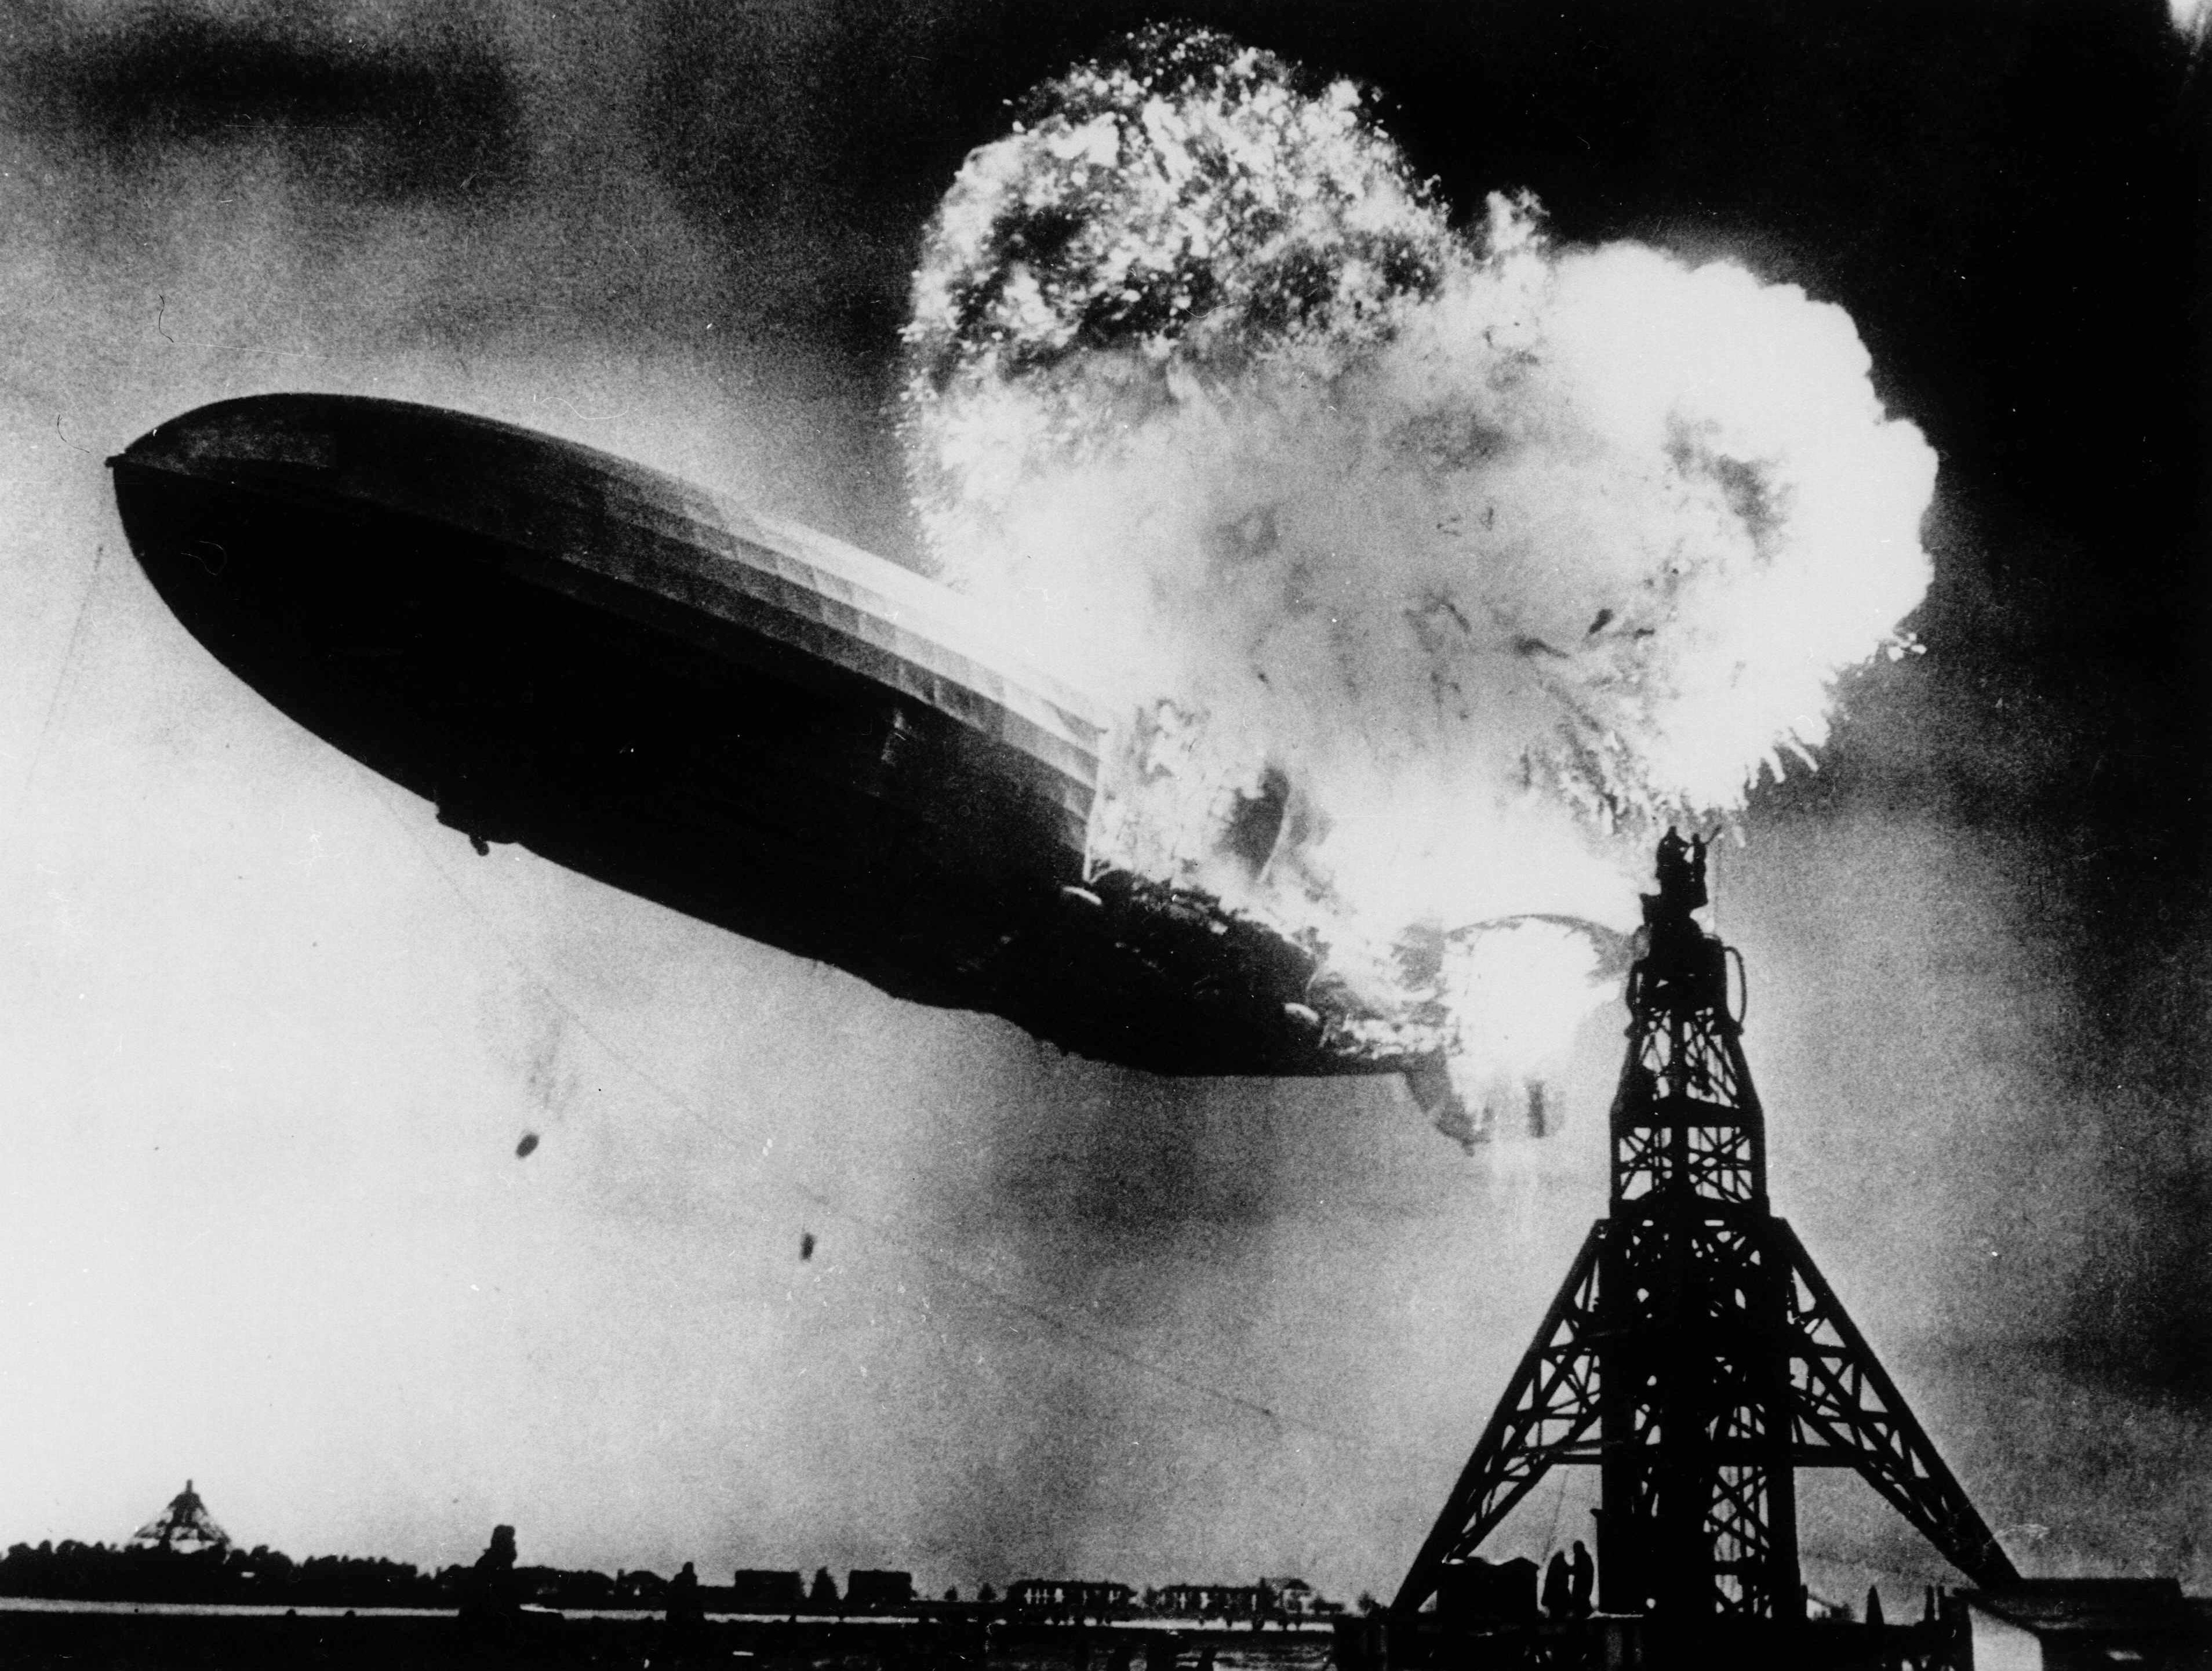
\includegraphics[width=4.0in]{diagrams/Hindenburg}
  \end{figure}
\end{frame}

\begin{frame}
  \frametitle{ Ethical Automation: Trust in Automation}
  {\Large Are we asking the right questions?}
  \begin{figure}[bht]
    \centering
    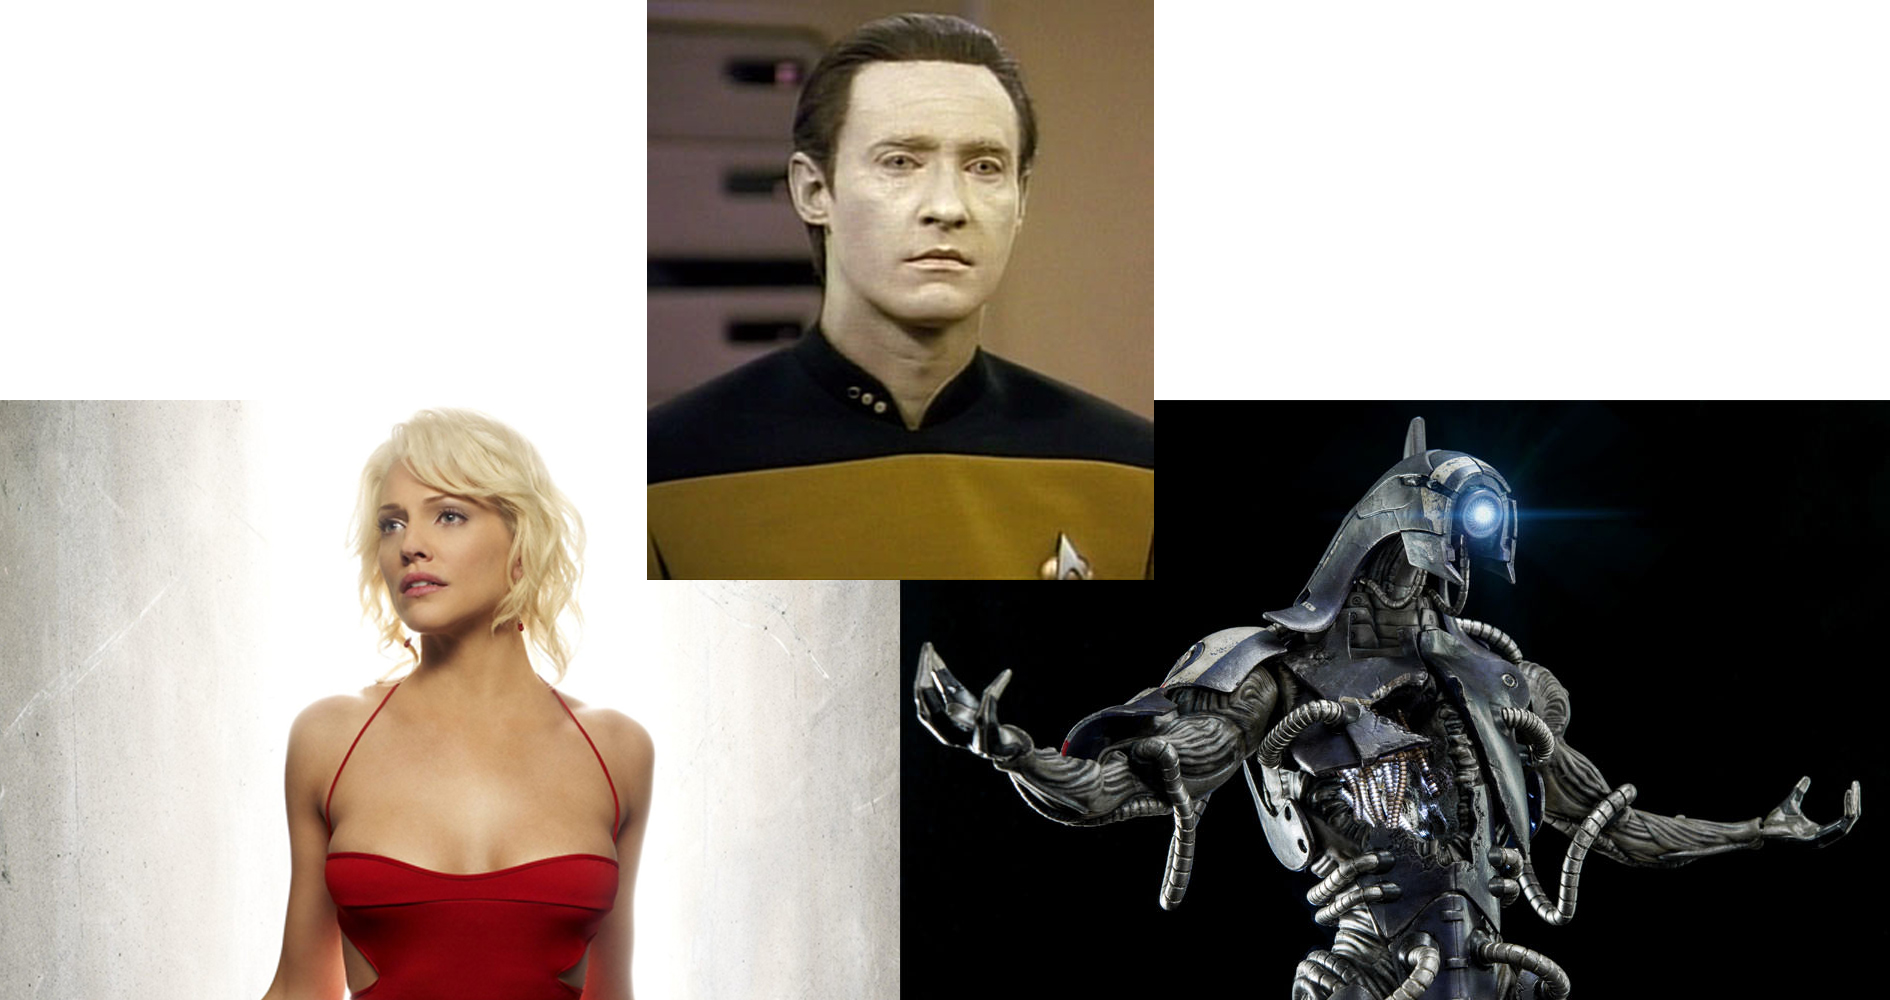
\includegraphics[width=4.0in]{diagrams/AIs}
  \end{figure}
\end{frame}

\begin{frame}
  \frametitle{ Ethical Automation: Conclusion}
  \begin{itemize}
    \item Consequences of automation
    \item Big changes are coming
      \begin{itemize}
        \item We've got to talk about it now,
        \item We've got to to talk about it a lot.
      \end{itemize}
  \end{itemize}
\end{frame}


\begin{frame}
  \frametitle{ Ethical Automation: Conclusion}
  \Large Questions?
\end{frame}

%%% Local Variables:
%%% mode: latex
%%% TeX-master: "main"
%%% End:
